
% Straight up stealing preamble from Eli Holmes 
%%%%%%%%%%%%%%%%%%%%%%%%%%%%%%%%%%%%%%START PREAMBLE THAT IS THE SAME FOR ALL EXAMPLES
\documentclass{article}[11pt]
%Required: You must have these
\usepackage{alltt}
\usepackage[margin=1in]{geometry}
\usepackage{graphicx}
\usepackage{natbib}
\usepackage{gensymb}
\begin{document}

\section*{Introduction}
\noindent Across the tree of life, temperature and light availability shape a number of important biological processes including growth and metabolics rates \citep{} sex determination \citep{}, acclimatization to seasonal environments \citep{} and the timing of life cycle transitions (phenology) \citep{}. These biological responses in turn dictate broad scale ecological processes and patterns ranging from biogeochemical cycling \citep{} to species range limits \citep{}.
A primary goal for research in of many sub-fields of biology is to characterize the the biological responses to varying enviornmental conditions.\\

%Characterizing the specific dynamics of how these environmental factors synergistically affect biological processes across a wide range of taxa has become even more important as anthropogenic global change continues to expose organisms to novel environmental conditions.\\

\noindent Because temperature and light availability often co-vary in the field (for example, in most temperate ecosystems, daylength and temperature both increase as the season progresses \citep{}) it is difficult to disentange their relative contributions to biological processes. Experimental manipulations of climate variables in artificial environments are ideal for mechanistically characterizing biological responses to environmental fluctuations \citep{Ettinger_inprep,Primack2015}. Growth chambers of all shapes and sizes have been used to this end \citep{} and these efforts have greatly advanced researchers understanding of the fundamental biology of a wide variety of organisms and their ability to predict the responses to current and future climate change. \citep{}.\\ 

\noindent Yet growth chamber studies come with their own unique set of challenges. When designing artificial environments, researcher must choose how many and which environmntal factors to vary, the intesity and periodicity of these treatments and the background levels of other environmental factors that are not being manipulated. Because biological responses to the environment are generally the product of complex interactions between multiple environmental signals \citep{}, these seeming small choices about experimental design can generate significant differences in outcomes, and as we demonstrate below, strongly bias the subsequent analyses. Experimental treatments appear to rarely be standardized among researchers even within disciplines \citep{} and these complexities may in part contribute to many discrepancies between experimental studies and observation data \citep{Poorter:2016aa}.\\

\noindent Even with these limitations, growth chamber studies remain a powerful tool for mechansitically assessing organismic responses to the environment provided that the implications of  treatment designs are well understood and well matched with the scope of the research question. Below, using plant phenology experiments as a case study, we discuss several common-use approaches to manipulating light and temperature in growth chamber studies. Need more here. %add a bit here

Here we focus our disucssion on the phenology of temperate woody plants, yet the insights of our case study can be readily applied to other study systems and biological processes.\\ 

\section*{Phenology, temperature and photoperiod}
\noindent Decades experimental work in growth chambers have demonstrated that temperature (winter chilling and spring forcing) and photoperiod are the primary cues of phenology for plants in the temperate/boreal zones \citep{}.  phenological responses to the environment tend to be nonlinear, due largely to interactions between two or more environmental cues\citep{Flynn2018,Laube2014}. From Drosophila \citep{Moghadam:2019aa,} to Arabidopsis, studies in model organisms suggest that these these environmental factors

highlighting the need for experiments to be designed to evaluate the strength of these interactions \citep{MacLean:2019aa}. Complex interactions 

To truly test interactions, treatments must be orthogonal: that is there must be more than one level of each treatment, and each level of each treatment must be crossed with every level of the other. While chilling is an important cue for spring phenology\citep{Ettinger2020} and interacts with other cues\citep{Flynn2018} , experiments apply chilling in complete darkness or approximate chilling by sequential field sampling dates so they are less prone to some of the complexities that arise under forcing and photperiod treatments. Because of this we focus our discussion on experiments that manipulate photoperiod and forcing condings, well recognizing that a good orthogial experiment will also include chilling treatments. \\

\noindent For both light and forcing cues, there are two axes that can be manipulated in experiments. Then intensity of the cue (ie temperature of forcing treamtent or intensity/wavelengthof the light treatment) and the period (duration of temperature exposure or light periods). While light intensity can affect phenology \citep{Brelsford2018,Cober1996}, period is considered to be the dominate light cue, and phenological research tends to focus on photoperiod rather than intensity (but see \citep{}). For temperature, intensity is an established driver of phenology, but the very common and successful modeling framework for quantifying temperature effects on phenology, the growing degree day or growing degree hour, integrates temperature with its period \citep{}. Seemingly simple decisions about how tovary photo-period and theromo-period relative to each other can disrupt the orthoginality of an experiment and add uncertainty to experimental results. Below we present three common approach to varying these three primary treatment axes (photo-period, theromo-period and thermo-intensity) in experiments, and discuss how each decision may affect experimental inferences.\\

\subsubsection*{Manipulation of Temperature intensity and photoperiod:}
\indent \indent The most simple design to test for a temperature x light interaction is to manipulate only one axis of each cue, for example, temperature intensity and light period. This would be implemented by applying high and low forcing treatments at constant temperatures, and crossing these with a long and short photo-period treatment at a constant light intensity (figure \ref{fig:Figure 1}a).\\
\indent The main advantage of this design is that is it simple to implement, maintains the orthogonality among the four treatment combinations (warm/short, warm/long, cool/short, cool/long) and allows for a very straightforward interpretation of the predictors. Additionally some studies have found that leaf expasion is faster at constant temperatures when compared to diurnally fluctation thermoperiods \citep{Erwin1995}. However,in nature, plants experience substantial diurnal temperature variation, and as such, growth chambers experiments without a diurnal thermoperiod would be a poor approximation of natural conditions. Other studies indicated that species may infact be responding to the differences between day and night temperatures \citep{Erwin1995},which raises futher questions about the utility experiments lacking thermoperiodicty for understanding the ecology and evolution of play in nature. On account of these shortcomings, it is more common for researchers to include a diurnally varying thermo-period for forcing treatments. For example, rather than static high/low forcing treatments of 20\degree C and 16\degree C, researchers would use, a high forcing treatment of 24\degree/16\degree C and low 20\degree/12\degree C (day/night).\\

\subsubsection*{Coupled photo- and thermo-periodicity:}
\indent\indent Incorporating diurnal thermo-periodicity into experimental design require that researcher decide how to vary this periodicity relative to the experiments photo-period cycle. The vast majority of published experiments employ a design in which photo-and thermo-periodicity are synchronized as in (figure \ref{fig:Figure 1}b) \citep{Ettinger_inprep}. This design is perhaps the most intuitive, one,  following the fact the photo- and thermo-period tend to co-vary in nature \citep{Rosenberg1974}. This approximation of natural conditions may make this design useful for extrapolating inferences between experimental and observational studies. However, while it appears, to maintain orthogonality between treatments when considering temperature intensity alone, but, in this case, the forcing response is a product of both the intensity of the temperature cue and the duration of its exposure (growing degree hours).  Thus, the coupling of photo- and thermo-period results in non-orthogonality between the four treatment combinations (see figure \ref{fig:Figure 2}). In this scenario, the effect of photo-period cannot be neatly distinguished from the effects of increased thermo-period under the longer day treatments, making it impossible to accurately evaluate the relative importance of these cues, which is often a a major goal of growth chamber experiments. This results in spurious interpretation of experimental results.\\

subsubsection*{Decoupled photo- and thermo-periodicity:}
 \indent \indent An alternative experimental design decouples the experimental thermo- and photo- periods. The would be achevied by varying thermo-period on a constant schedule across all four treatment combinations (figure \ref{fig:Figure 1}c). Though this experiment set up has not be widely employed in growth chamber experiments (but see \citep{Buonaiuto2020}), this design restores full orthogonality to growing degree hour sums that make up the forcing treatment (figure \ref{fig:Figure 2}a).\\
 
\noindent But this obvious advantage for reasonible statistical comparisons introduces a new biological artifact that may bias experimental results. Evidence from horticulture studies have demonstrated that cell growth is most sensitive to temperature fluctuation at the beginning of the photoperiod\citep{Erwin1998}. \citet{Erwin1998} found that increasing temperatures in the first two hours of the photoperiod was almost as effective for stimulating shoot elongation as similar temperature increases for the whole photoperiod. More generally, recenty work suggests that phenology is more responsive to daytime warming that night \citep{Rossi2017}. By de-coupling thermo-period from the photo-period manipulations, experimenters by neccesity introduce an assymetry between the photoperiod treatments \textit{relative} to the thermo-period. In our example in \ref{fig:Figure 1}c), the long and short day photoperiod treatments have the same 12 thermoperiodicity cycle, but in the long day treatments, the plant does not experience "day time" temperatures until after they encounter "day light", while the plants in the short day treatment experience day time warming before light.\\

\noindent One solution to this problem is a modified decoupled design where the decouping of thermo- and photo periodicty happens in the evening \ref{fig:Figure 1}d in and improved version of a uncouple thermo and photo period design, because the temporal relationship between dawn light and temperature is standardized across all treatments, but this again produces an unreasilstic comparision with nature, and the "true" effects of warming may be obscured by that fact for the short day treatments, there is less overlap between day time temperature and light conditions.\\ %%% I am acutally slowly convincing myself that this design is superior and should be used

\indent As we have shown above, each design introduces its own biological or statistical artifacts that will bias he results of the experiments. We cannot conclusively solve the problems of true inference through modifying experimental designs, but rather, we must thoughtful incorporate the implications of these design choices into our statistical metrics and interpretation of results.\\ 

\noindent While each design has a tradeoff we expect that a coupled photo-and thermo- period design will remain the most popular choice for phenological experiments in artificial environments. In the following section, we will use a public dataset to demonstrate how mathematical principles can be applied to tease apart the artifact introduced by this inherently imperfect experimental design and make more meaningful inferences about the cue interactions. 

\section*{Theoretical evidence}   
\noindent The following analysis is based on results from a large scale growth chamber experiment by \citet{Flynn2018}, in which in addition to chilling and provenance, fully factorial light and temperature manipulations were applied to twig cuttings from 28 woody species. 
The authors applied two photoperiods (12 and 8 hours) crossed with 2 dirunally fluctuating temperature treamtments (20/10\degree and 15/5\degree) in which the thermo-periodicity was coupled with the photo-periodicity.\\ 

The authors estimated a budburst sensitive to forcing of -9  a mean sensitivity to photo-period of -4.5 with a weak interaction between the two cues. We can treat the interaction term as 0, and then using fact the the photoperiod and forcing model estimates are additive, we can convert the temperature treatments into growing degree hours and calculate the estimated effects of the treatment combinations.

$short photoperiod* warm temperatures =(20\degree)*(8 hrs) + 10\degree*(16 hrs)= 320 GDH$\\ 
$estimate effect size = 0_{photoperiod} + 9+{forcing} = 9\\
$short photoperiod* cool temperatures =(15\degree)*(8 hrs) + 5\degree*(16  hrs)= 200 GDH$ \\
$long photoperiod* warm temperatures =(20\degree)*(12 hrs) + 10\degree*(12 hrs)= 360 GDH$\\ 
$estimate effect size = 0_{photoperiod} + 9+{forcing} = 9\\
$long photoperiod* cool temperatures =(15\degree)*(12 hrs) + 5\degree*(12  hrs)= 240 GDH$ \\

From these conversions we can estimate a plane ax+by+cz+d=0\\
Our goal is to estimate d but Im not sure what that is.\\
 With the following system of equations we can solve for d in each case and use the fourth to check.




We set out to calculate how much of the reported photo-period response could in actuality be driven by the unaknowledged differences in thermo-period between the long and short photo-period treatments. \\

\noident Our analysis rests on several assumtions. First, we assume that following the phenology literature forcing is a more dominate cue than photoperiod \citep{}. This suggests that if anything, they photoperiod cue will be over-estimated due to the differences in thermo-period as opposed to the other way around. Second because the authors only report a weak interactions between these two cues, we treat these reponses as additive. Third, we assume we assume these cues are linear.\\

Math here

\section*{Experimental comparison}
\indent\indent Our prediction of ``how much of the reported photo-period response could in actuality be driven by the unaknowledged differences in thermo-period" can be rephrased as a prediction of the expected difference in estimated photoperiod sensitivity between a coupled and decoupled photo- and thermo-period experiment. While we are aware of no experiments that explicitly test these different designs, we now present an additional growth chamber data set from  \citet{Buonaiuto2020} that allows us to empirical test our predictions. The \citet{Buonaiuto} study applied serveral treatments levels that overlap with those in the \citet{Flynn2018} study to twig cuttings from the same source population. However in the second study the authors decoupled photo- and thermo-period. We subset each dataset to only include species and treatment levels common amoung them, and combined and re-analysized them in a model that estimated differences in the photo-period effect between the two studies. We found that the estimated difference in the average response to photoperiod amoung study designs  was on the same order our mathmatical prediction.\\

\section*{Moving forward}
\begin{enumerate}
\item What to say here
\end{enumerate}

\bibliography{..//refs/periodicity.bib} 

\begin{figure}[h!]
    \centering
 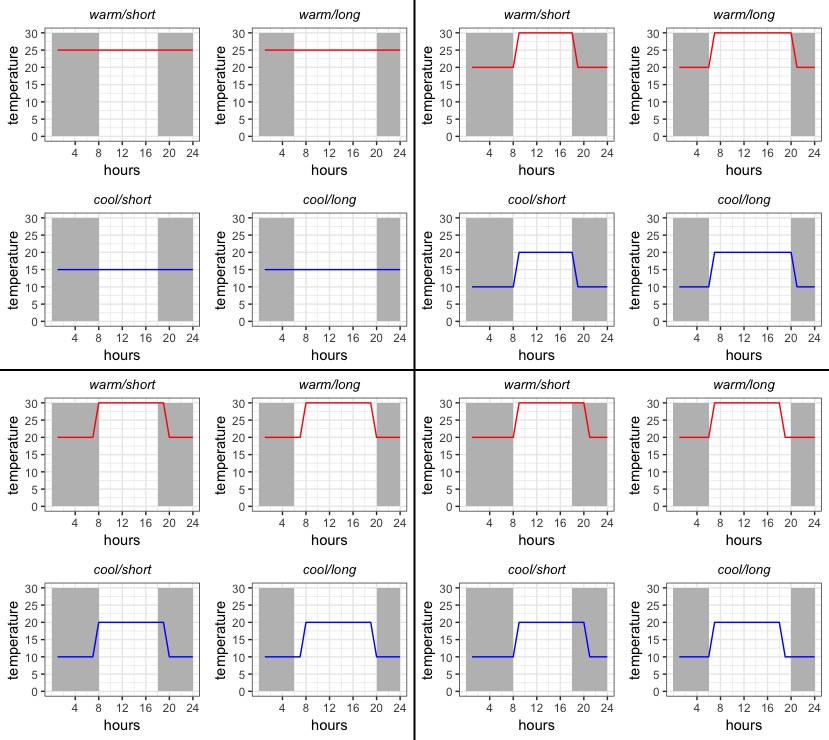
\includegraphics[width=\textwidth]{..//Plots/periodicity_figures/new_treats.jpeg}
    \caption{Experimental treatments}
    \label{fig:Figure 1}
\end{figure}

\begin{figure}[h!]
    \centering
 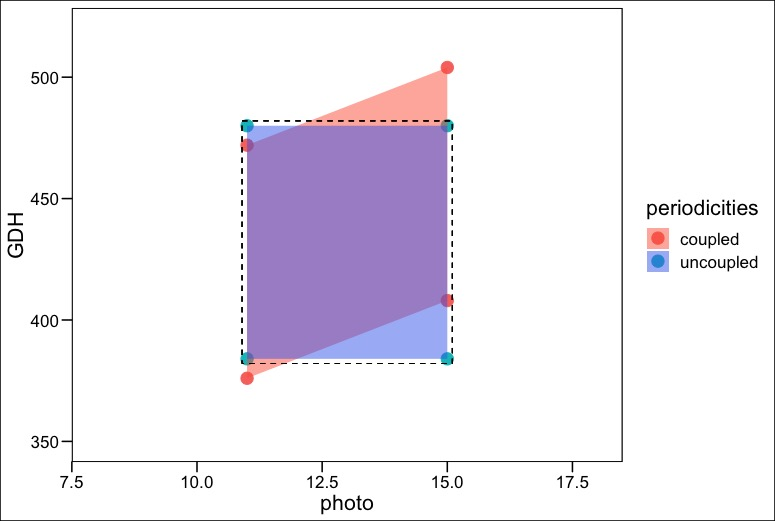
\includegraphics[width=\textwidth]{..//Plots/periodicity_figures/Uncoupled_coupled.jpeg}
    \caption{Experimental comparison all species}
    \label{fig:Figure 2}
\end{figure}

\begin{figure}[h!]
    \centering
 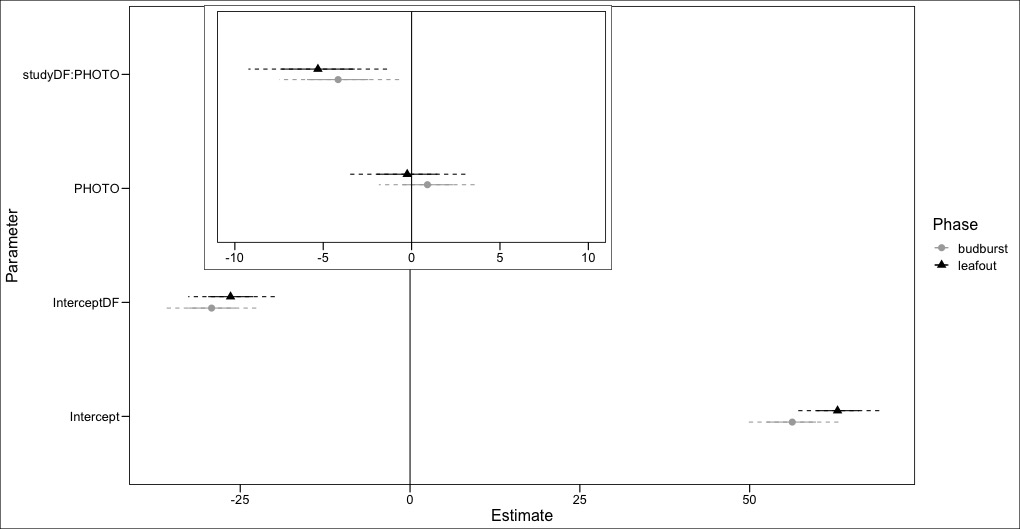
\includegraphics[width=\textwidth]{..//Plots/periodicity_figures/photothermo_allsps.jpeg}
    \caption{All species with partial pooling}
    \label{fig:Figure 3}
\end{figure}


\begin{figure}[h!]
    \centering
\begin{tabular}{|c|c|c|}
\hline
& predicted difference & observed difference (sd)\\
\hline
bud bust& 3.0 & -4.1575777(2.665567)\\
leaf out&3.0 & -5.3006250 (3.099359)\\
\hline
\end{tabular}
    \caption{Table}
    \label{fig:Figure 4}
\end{figure}






\end{document}